% Preamble
% ---
\documentclass[a4paper]{article}

% Packages
% ---
\usepackage{bm}
\usepackage[spanish,es-nodecimaldot]{babel}
\usepackage[utf8]{inputenc}
\usepackage[T1]{fontenc}
\usepackage{parskip}
\usepackage{fancyhdr}
\usepackage{mathtools}
\usepackage{amsmath}
\usepackage[htt]{hyphenat}
\usepackage{capt-of}
\usepackage{changepage}
\usepackage{graphicx}
\graphicspath{ {./images/} }

% Pagestyles
% ---
\pagestyle{fancy}
\rhead{Roselló Beneitez, N. U.; Roselló Oviedo, M.}
\lhead{APR: Práctica sobre MLP}
\fancyfoot[C]{\thepage}

% Main
% ---
\begin{document}

\author{Roselló Beneitez, N. U.; Roselló Oviedo, M.}
\title{APR: Práctica sobre Redes Neuronales Multicapa (MLP)}
\date{6 de Enero de 2020}
\maketitle{}
\thispagestyle{empty}

\newpage
\tableofcontents
\listoffigures

\newpage
\section{Descripción de la práctica}
\quad En esta práctica se ha trabajado con redes neuronales multicapa en Octave mediante la librería \textit{nnet}, la cual dispone de sus propios métodos auxiliares con los que entrenar un \textit{multilayer perceptron}.

\quad La primera parte de la práctica, de carácter didáctico e iniciativo, consiste en experimentar con el corpus \textit{hart} para familiarizarse con la metodología de la librería, y no se halla incluida en esta memoria. La segunda parte, la cual desarrollaremos a continuación, se centra en la clasificación de dígitos de la base de datos MNIST.

\section{Redes neuronales en MNIST}
\quad Se ha entrenado la red neuronal con diversos valores de porcentaje de muestras destinadas al entrenamiento, concretamente 50\% y 80\%; el resto de los valores de entrenamiento se han destinado al conjunto de validación del modelo.

\quad Puesto que los recursos de los equipos disponibles no eran ilimitados, han habido ejecuciones para las que no ha sido posible obtener un resultado, bien porque el entrenamiento ha sido terminado por el programa en el entrenamiento, o bien porque no se disponía de la suficiente memoria RAM como para almacenar todos los cálculos en memoria, por lo que el programa utilizaba memoria virtual procedente del disco y como consecuencia el tiempo del entrenamiento aumentaba de manera drástica.

\quad Para ambos porcentajes de entrenamiento, se han realizado experimentos variando tanto la reducción de dimensionalidad mediante PCA como el número de neuronas en la capa oculta (todos los experimentos cuentan con una sola capa oculta). El error obtenido se muestra en cada correspondiente casilla de las tablas siguientes tablas.

\subsection{Entrenamiento con 50\%}

\quad En primer lugar, con un 50\% de muestras destinadas a entrenamiento el mejor error es de un 4.28\% al emplear 40 neuronas en la capa oculta y 30 dimensiones de PCA.
$ \\ $
\begin{center}
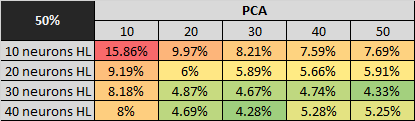
\includegraphics[width=250px]{3_50_tabla}
\captionof{figure}{{\footnotesize Error en función de PCA y número de neuronas, usando el 50\% de las muestras para entrenamiento.}}
\end{center}
$ \\ $
\begin{center}
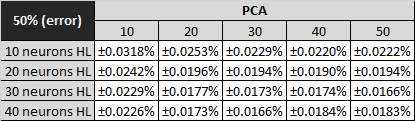
\includegraphics[width=250px]{3_50_error}
\captionof{figure}{{\footnotesize Intervalos de confianza para el experimento de 50\%.}}
\end{center}
$ \\ $
\subsection{Entrenamiento con 80\%}

\quad El segundo experimento, con 80\% de muestras para entrenamiento, produjo mejores resultados, con un mínimo de 3.40\% para los mismos parámetros que el caso anterior.
$ \\ $
\begin{center}
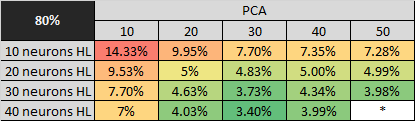
\includegraphics[width=250px]{3_80_tabla}
\captionof{figure}{{\footnotesize Error en función de PCA y número de neuronas, usando el 80\% de las muestras para entrenamiento.}}
\end{center}
$ \\ $
\begin{center}
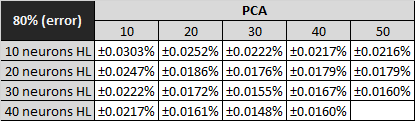
\includegraphics[width=250px]{3_80_error}
\captionof{figure}{{\footnotesize Intervalos de confianza para el experimento de 80\%.}}
\end{center}
$ \\ $

\newpage
\subsection{Comparativa}

A continucación se pueden observar las gráficas respresentando los resultados para cada experimento:

\begin{figure}[!h]
	\begin{adjustwidth}{-70pt}{-70pt}
	  \centering
	  \begin{minipage}[b]{0.65\textwidth}
	    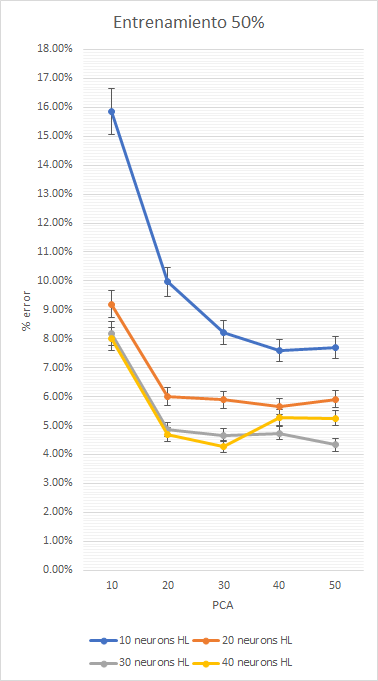
\includegraphics[width=\textwidth]{3_50_graph}
	    \caption{{\footnotesize Visualización gráfica de los resultados para 50\%.}}
	  \end{minipage}
	  \hfill
	  \begin{minipage}[b]{0.65\textwidth}
	    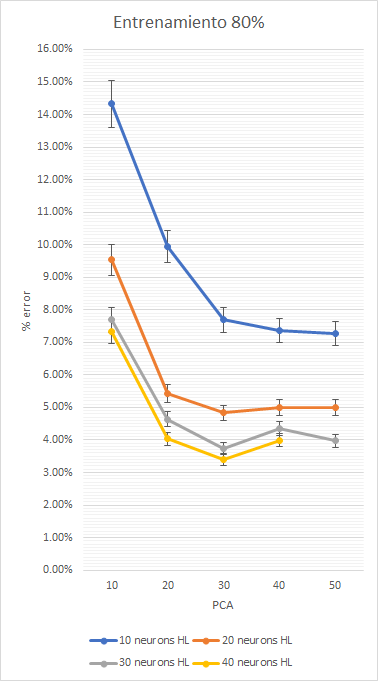
\includegraphics[width=\textwidth]{3_80_graph}
	    \caption{{\footnotesize Visualización gráfica de los resultados para 80\%.}}
	  \end{minipage}
	  \end{adjustwidth}
\end{figure}


\newpage
Finalmente, se ha realizado una tabla comparativa para facilitar la visualización de todos los resultados.
$ \\ $
\begin{center}
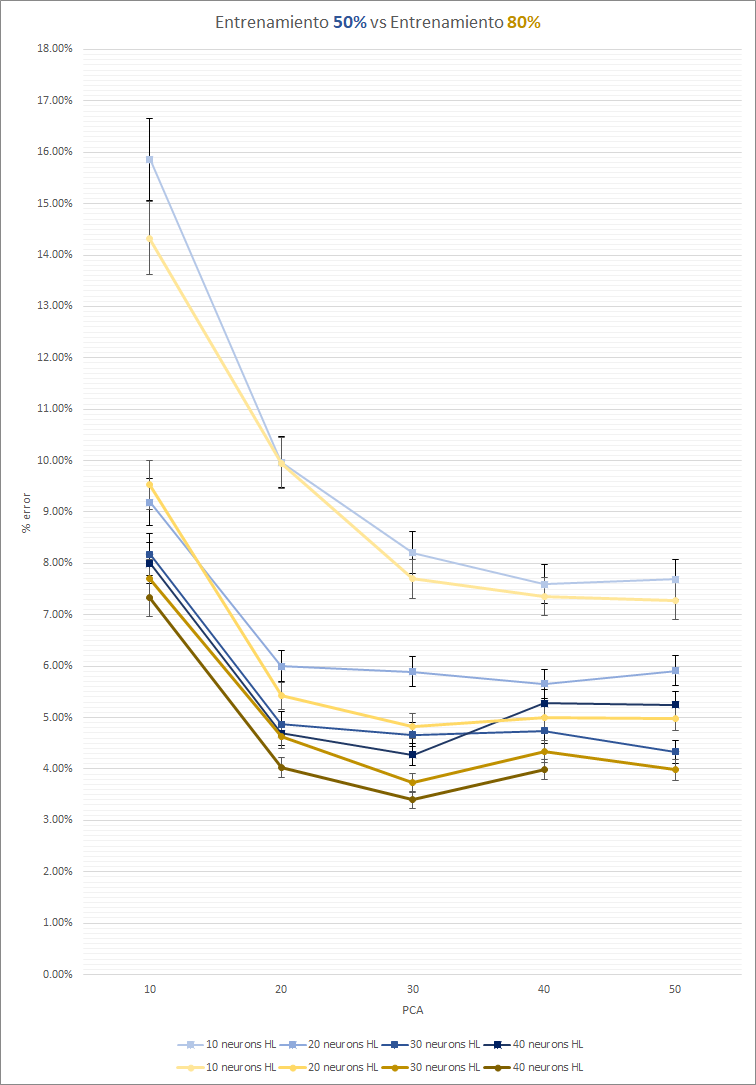
\includegraphics[width=\textwidth]{3_comparativa}
\captionof{figure}{{\footnotesize Comparativa de los resultados para 50\% vs 80\%.}}
\end{center}

\section{Conclusiones}
\quad Como se puede ver cuando se analizan los porcentajes de error y los intervalos de confianza, la mayoría de los errores presentan una diferencia estadísticamente significativa usando el 80\% de las muestras para entrenamiento con respecto a usar el 50\% de muestras. Esto indica, como parece lógico, que es útil tener un porcentaje más elevado dedicado al entrenamiento que a la validación, lo cual tiene sentido ya que al introducir más muestras en el conjunto de validación se están desaprovechando muestras perfectamente válidas para el entrenamiento. Según lo visto en la teoría, el conjunto de validación debería establecer cuándo se pasa de generalizar a sobreentrenar el modelo, por lo que en nuestra opinión un conjunto tan grande como el de pruebas debería ser suficiente en la mayoría de los casos para evitar un desaprovechamiento de los datos de entrenamiento. Cabe recordar que en nuestras ejecuciones el tamaño del conjunto de validación era de 30000 y de 12000 muestras, esto es, un 50\% y un 20\% del conjunto de entrenamiento respectivamente.

\quad Con respecto a la variación del error con respecto al número de dimensiones proyectadas con PCA y al número de neuronas en la capa oculta, se puede ver un descenso notable del error a medida que tanto las dimensiones proyectadas con PCA como el número de neuronas en la capa oculta aumenta. No es beneficioso para el modelo, sin embargo, aumentar el número de una de estas dos componentes manteniendo la otra marginalmente mínima, como se puede apreciar en las tablas obtenidas. Lo óptimo es encontrar un balance entre ambas componentes: el mejor resultado del error para cada porcentaje de entrenamiento coincide en ser aquel obtenido mediante 40 neuronas en la capa oculta y la proyección a 30 dimensiones con PCA para el conjunto de entrenamiento, tanto al 50\% (con error 4.28\%) y al 80\% (con error 3.40\%), respectivamente.

\quad Por último, cabe mencionar que el modelo conexionista no siempre es la solución óptima a todos los problemas. La menor tasa de error encontrada ha sido de un 3.40\%, mientras que las tasas de error encontradas en prácticas anteriores han sido de un 2.20\% para la \textit{Práctica 1 sobre Mixtura de gaussianas} y de un 1.95\% para la \textit{Práctica 2 sobre Máquinas de vector soporte}. Esto no quiere decir que estas dos técnicas sean mejores que las redes neuronales, sino que son mejores \textit{para este problema específico de clasificación de dígitos}. Es por esto que es necesario un cierto conocimiento experto sobre las técnicas de aprendizaje automático, además de los mejores \textit{toolkits} que las implementan, con el fin de saber cuáles son sus mejores aplicaciones.

\end{document}
